\documentclass[11pt,a4paper]{article}
\pdfoutput=1
\usepackage{jinstpub}

%\usepackage{draftwatermark}

\newcommand{\ignore}[1]{}
%\renewcommand*\contentsname{Table of Contents}
\newcommand\todo[1]{}
\newcommand\stub[1]{\input{#1}}

% side-by-side figures
\usepackage{caption}
\usepackage{subcaption}

%%% Needed to make subsubsubsubsections...
\usepackage{titlesec}
\usepackage{multirow}
\usepackage{booktabs}
\usepackage{bm}
\usepackage{fancyhdr}
\usepackage{color}
\usepackage{graphicx}

\pagestyle{fancy}
%%% How deep do we count in ``sub''sections...
\setcounter{secnumdepth}{4}
%%% These lines do the re-purposing of paragraph into ``subsubsubsubsection''
\titleformat{\paragraph}
{\normalfont\normalsize\bfseries}{\theparagraph}{1em}{}
\titlespacing*{\paragraph}
{0pt}{3.25ex plus 1ex minus .2ex}{1.5ex plus .2ex}

%\renewcommand{\baselinestretch}{0.965}

% Some neutrino physics shortcuts
\newcommand{\nua}{\ensuremath{\nu_\alpha}\xspace}
\newcommand{\nub}{\ensuremath{\nu_\beta}\xspace}
\newcommand{\nue}{\ensuremath{\nu_e}\xspace}
\newcommand{\num}{\ensuremath{\nu_{\mu}}\xspace}
\newcommand{\nut}{\ensuremath{\nu_{\tau}}\xspace}
\newcommand{\nuabar}{\ensuremath{\bar{\nu}_\alpha}\xspace}
\newcommand{\nubbar}{\ensuremath{\bar{\nu}_\beta}\xspace}
\newcommand{\nuebar}{\ensuremath{\bar{\nu}_e}\xspace}
\newcommand{\numbar}{\ensuremath{\bar{\nu}_{\mu}}\xspace}
\newcommand{\nutbar}{\ensuremath{\bar{\nu}_{\tau}}\xspace}

\title{Deep Learning in Liquid argon time projection chambers: Optimizing the Architecture for Particle Classification}
\collaboration{MicroBooNE Collaboration}

\abstract{
Liquid Argon Time Projection Chambers (LArTPCs) produce image-like data that may be analyzed with deep neural networks (Deep Learning, or DL). This approach to data analysis is becoming more common in LArTPCs, as well as other high channel-count segmented detectors where events may be interpreted as images. In particular, MicroBooNE is an 8256 wire detector viewing 89 tons of fiducial liquid argon, where studies have demonstrated single particle classification capability using DL as well as progress toward DL neutrino identification \cite{uB-JINST}. In the case of these previous studies, the performance dependence on a variety of network architecture types was not explored in great depth.  Using the same single particle classification metric, this paper seeks to provide a baseline of guidance for choosing the optimal network for the task at hand.  We answer key questions about performance as a function of network architectures and show that networks \_\_, \_\_ and \_\_ give functionally equivalent high performance, with gains in network \_\_ in resource consumption that suggest its use.
}

\begin{document}
% Authors in alphabetical order
\author[g]{R.~Acciarri}
\author[z]{C.~Adams}
\author[h]{R.~An}
\author[w]{J.~Asaadi}
\author[a]{M.~Auger}
\author[g]{L.~Bagby}
\author[g]{B.~Baller}
\author[q]{G.~Barr}
\author[q]{M.~Bass}
\author[x]{F.~Bay}
\author[b]{M.~Bishai}
\author[j]{A.~Blake}
\author[i]{T.~Bolton}
\author[m]{L.~Bugel}
\author[f]{L.~Camilleri}
\author[f]{D.~Caratelli}
\author[g]{B.~Carls}
\author[g]{R.~Castillo~Fernandez}
\author[g]{F.~Cavanna}
\author[b]{H.~Chen}
\author[r]{E.~Church}
\author[l,f]{D.~Cianci}
\author[m]{G.~H.~Collin}
\author[m]{J.~M.~Conrad}
\author[u]{M.~Convery}
\author[f]{J.~I.~Crespo-Anad\'{o}n}
\author[q]{M.~Del~Tutto}
\author[j]{D.~Devitt}
\author[s]{S.~Dytman}
\author[u]{B.~Eberly}
\author[a]{A.~Ereditato}
\author[c]{L.~Escudero Sanchez}
\author[v]{J.~Esquivel}
\author[z]{B.~T.~Fleming}
\author[d]{W.~Foreman}
\author[l]{A.~P.~Furmanski}
\author[k]{G.~T.~Garvey}
\author[f]{V.~Genty}
\author[a]{D.~Goeldi}
\author[i]{S.~Gollapinni}
\author[s]{N.~Graf}
\author[z]{E.~Gramellini}
\author[g]{H.~Greenlee}
\author[e]{R.~Grosso}
\author[q]{R.~Guenette}
\author[z]{A.~Hackenburg}
\author[v]{P.~Hamilton}
\author[m]{O.~Hen}
\author[l]{J.~Hewes}
\author[l]{C.~Hill}
\author[d]{J.~Ho}
\author[i]{G.~Horton-Smith}
\author[g]{C.~James}
\author[c]{J.~Jan~de~Vries}
\author[y]{C.-M.~Jen}
\author[s]{L.~Jiang}
\author[e]{R.~A.~Johnson}
\author[m]{B.~J.~P.~Jones}
\author[b]{J.~Joshi}
\author[g]{H.~Jostlein}
\author[f]{D.~Kaleko}
\author[l,f]{G.~Karagiorgi}
\author[g]{W.~Ketchum}
\author[b]{B.~Kirby}
\author[g]{M.~Kirby}
\author[g]{T.~Kobilarcik}
\author[a]{I.~Kreslo}
\author[q]{A.~Laube}
\author[b]{Y.~Li}
\author[j]{A.~Lister}
\author[h]{B.~R.~Littlejohn}
\author[g]{S.~Lockwitz}
\author[a]{D.~Lorca}
\author[k]{W.~C.~Louis}
\author[a]{M.~Luethi}
\author[g]{B.~Lundberg}
\author[z]{X.~Luo}
\author[g]{A.~Marchionni}
\author[y]{C.~Mariani}
\author[c]{J.~Marshall}
\author[h]{D.~A.~Martinez~Caicedo}
\author[i]{V.~Meddage}
\author[o]{T.~Miceli}
\author[k]{G.~B.~Mills}
\author[m]{J.~Moon}
\author[b]{M.~Mooney}
\author[g]{C.~D.~Moore}
\author[n]{J.~Mousseau}
\author[l]{R.~Murrells}
\author[s]{D.~Naples}
\author[t]{P.~Nienaber}
\author[j]{J.~Nowak}
\author[g]{O.~Palamara}
\author[s]{V.~Paolone}
\author[o]{V.~Papavassiliou}
\author[o]{S.F.~Pate}
\author[g]{Z.~Pavlovic}
\author[l]{D.~Porzio}
\author[v]{G.~Pulliam}
\author[b]{X.~Qian}
\author[g]{J.~L.~Raaf}
\author[i]{A.~Rafique}
\author[u]{L.~Rochester}
\author[a]{C.~Rudolf~von~Rohr}
\author[z]{B.~Russell}
\author[d]{D.~W.~Schmitz}
\author[g]{A.~Schukraft}
\author[f]{W.~Seligman}
\author[f]{M.~H.~Shaevitz}
\author[a]{J.~Sinclair}
\author[g]{E.~L.~Snider}
\author[v]{M.~Soderberg}
\author[l]{S.~S{\"o}ldner-Rembold}
\author[q]{S.~R.~Soleti}
\author[g]{P.~Spentzouris}
\author[n]{J.~Spitz}
\author[e]{J.~St.~John}
\author[g]{T.~Strauss}
\author[l]{A.~M.~Szelc}
\author[p]{N.~Tagg}
\author[f]{K.~Terao}
\author[c]{M.~Thomson}
\author[g]{M.~Toups}
\author[u]{Y.-T.~Tsai}
\author[z]{S.~Tufanli}
\author[u]{T.~Usher}
\author[k]{R.~G.~Van~de~Water}
\author[b]{B.~Viren}
\author[a]{M.~Weber}
\author[c]{J.~Weston}
\author[s]{D.~A.~Wickremasinghe}
\author[r]{K.~Wierman}
\author[g]{S.~Wolbers}
\author[m]{T.~Wongjirad}
\author[o]{K.~Woodruff}
\author[g]{T.~Yang}
\author[g]{G.~P.~Zeller}
\author[d]{J.~Zennamo}
\author[b]{C.~Zhang}

% Institutions in alphabetical order
\affiliation[a]{Universit{\"a}t Bern, Bern CH-3012, Switzerland}
\affiliation[b]{Brookhaven National Laboratory (BNL), Upton, NY, 11973, USA}
\affiliation[c]{University of Cambridge, Cambridge CB3 0HE, United Kingdom}
\affiliation[d]{University of Chicago, Chicago, IL, 60637, USA}
\affiliation[e]{University of Cincinnati, Cincinnati, OH, 45221, USA}
\affiliation[f]{Columbia University, New York, NY, 10027, USA}
\affiliation[g]{Fermi National Accelerator Laboratory (FNAL), Batavia, IL 60510, USA}
\affiliation[h]{Illinois Institute of Technology (IIT), Chicago, IL 60616, USA}
\affiliation[i]{Kansas State University (KSU), Manhattan, KS, 66506, USA}
\affiliation[j]{Lancaster University, Lancaster LA1 4YW, United Kingdom}
\affiliation[k]{Los Alamos National Laboratory (LANL), Los Alamos, NM, 87545, USA}
\affiliation[l]{The University of Manchester, Manchester M13 9PL, United Kingdom}
\affiliation[m]{Massachusetts Institute of Technology (MIT), Cambridge, MA, 02139, USA}
\affiliation[n]{University of Michigan, Ann Arbor, MI, 48109, USA}
\affiliation[o]{New Mexico State University (NMSU), Las Cruces, NM, 88003, USA}
\affiliation[p]{Otterbein University, Westerville, OH, 43081, USA}
\affiliation[q]{University of Oxford, Oxford OX1 3RH, United Kingdom}
\affiliation[r]{Pacific Northwest National Laboratory (PNNL), Richland, WA, 99352, USA}
\affiliation[s]{University of Pittsburgh, Pittsburgh, PA, 15260, USA}
\affiliation[t]{Saint Mary's University of Minnesota, Winona, MN, 55987, USA}
\affiliation[u]{SLAC National Accelerator Laboratory, Menlo Park, CA, 94025, USA}
\affiliation[v]{Syracuse University, Syracuse, NY, 13244, USA}
\affiliation[w]{University of Texas, Arlington, TX, 76019, USA}
\affiliation[x]{TUBITAK Space Technologies Research Institute, METU Campus, TR-06800, Ankara, Turkey}
\affiliation[y]{Center for Neutrino Physics, Virginia Tech, Blacksburg, VA, 24061, USA}
\affiliation[z]{Yale University, New Haven, CT, 06520, USA}

\maketitle
%\tableofcontents

\thispagestyle{empty}


\arxivnumber{1234.56789} 

\pagenumbering{arabic}

%\cleardoublepage
\setcounter{page}{1}
\newpage

%% Project Narrative %%
\section{Introduction}

MicroBooNE is the first large-scale LArTPC detector to collect data in a neutrino beam in the United States. The experiment has a total liquid argon mass of 170 tons and a rectangular active volume of 2.3$\times$2.6$\times$10.4 m$^3$. The system consists of two subdetectors: a time projection chamber (TPC) for tracking and calorimetry along with a light collection system for the detection of scintillation light.  The detector began observing interactions of neutrinos from the FNAL Booster Neutrino Beam (BNB)~\cite{BNB} in October, 2015.

The information we consider in these performance studies is TPC readout only. Here, TPC information comes in the form of 3 wire readout planes, where each plane represents 1 image.  Unlike the images normally used in image classification tasks, MicroBooNE's images are sparse; this means that most of the roughly 9600x3000 image pixels are at their pedestal value for each event. The complications and final handling of such sized images is discussed in detail in a previous paper \cite{uB-JINST}. A typical event is shown in Figure~\ref{fig:UBEVD}.

%In this paper we will survey the performance of various networks on image detection in LArTPCs. 
%Tracks, showers and isolated electromagnetic activity produce a relatively small fraction of pixels that are activated in LArTPCs. This is true even for MicroBooNE's particular case in which the detector sits on the surface and sees a $\approx 5 $ kHz of through-going cosmic rays and associated activity.

In this paper, we survey variants of 2 well-used networks in image recognition literature: ResNet ~\cite{} and Vgg16 ~\cite{}. We are interested in both their parameters and architectures, which means we will explore the depth and width of these networks, the addition of fully connected layers, stride sizes, input sparsification, and ``bottlenecks.''  We seek to understand whether or not networks that are less computationally expensive can match their more expensive counterpart networks in performance, in addition to seeking highest classification performance. 
%and thus might be used in their place.


The organization of this paper consists of a description of our single particle metrics, the preparation of the images, the training and inference protocol used, and finally a description of the various architectures with results, followed by conclusions.

\begin{figure}[t]
  \centering  
%\includegraphics[width=0.495\textwidth]{section2/run3469_subrun574_event28734_ind0.pdf}\\
%\includegraphics[width=0.495\textwidth]{section2/run3469_subrun574_event28734_ind1.pdf}\\
%\includegraphics[width=0.495\textwidth]{section2/run3469_subrun574_event28734_col.pdf}\\
\caption{Example neutrino candidate observed in the MicroBooNE detector.  The same interaction is shown in all three wire plane views.  The top image is from wire plane $U$; the middle from wire plane $V$; and the bottom from wire plane $Y$. The image is at full resolution and is only from a portion of the full event view.}
  \label{fig:UBEVD}
\end{figure}


%{\color{red} Outline roughly from 
%\begin{verbatim}https://docs.google.com/https://docs.google.com/document/d/1HalATQK5RneLrzhL2Tk-n-c1jI-7hXnXBNunSb13dQY
%\end{verbatim} }

\section{Particle Classification}

In this paper we study the performance of five particle classification ($e^-$, $\gamma$, $\mu^-$, $\pi^-$, proton) using a variety of Convolutional Neural Networks (CNNs). We simulate these particles in the 50-500 MeV/c momentum range of interest to MicroBooNE using the relevant Geant4-based LArSoft package~\cite{larsoft050800}.  The $e^-$ and $\gamma$ are electromagnetic particles that develop as showery objects in the detector. These are generally distinguishable by eye from their $\mu^-$, $\pi^-$ and proton track-like counterparts, which form more linear traces in the detector.  The networks learn these features and others to make final identification. Such other distinguishing characteristics include $dQ/ds$ variation at track ends (Bragg peak) and total $Q$ deposition differences, per the Bethe-Bloch curves for different particle species.  We note, however, that unlike a more traditional case of cat, dog, human-face image data separation, we are faced with some level of irreducible ambiguity in our five particle classification. In particular, $\mu^-$'s and $\pi^-$s are minimum-ionizing particles which will only be discernable in the cases that, say, the $\mu^-$ captures or the $\pi^-$ scatters and produces a kink or inelastic interaction. Additionally, sometimes the simulated $\pi^-$ will even decay to a $\mu^-$.  Therefore, we expect lower separation power between these particular species.

\begin{figure}[t]
  \centering  
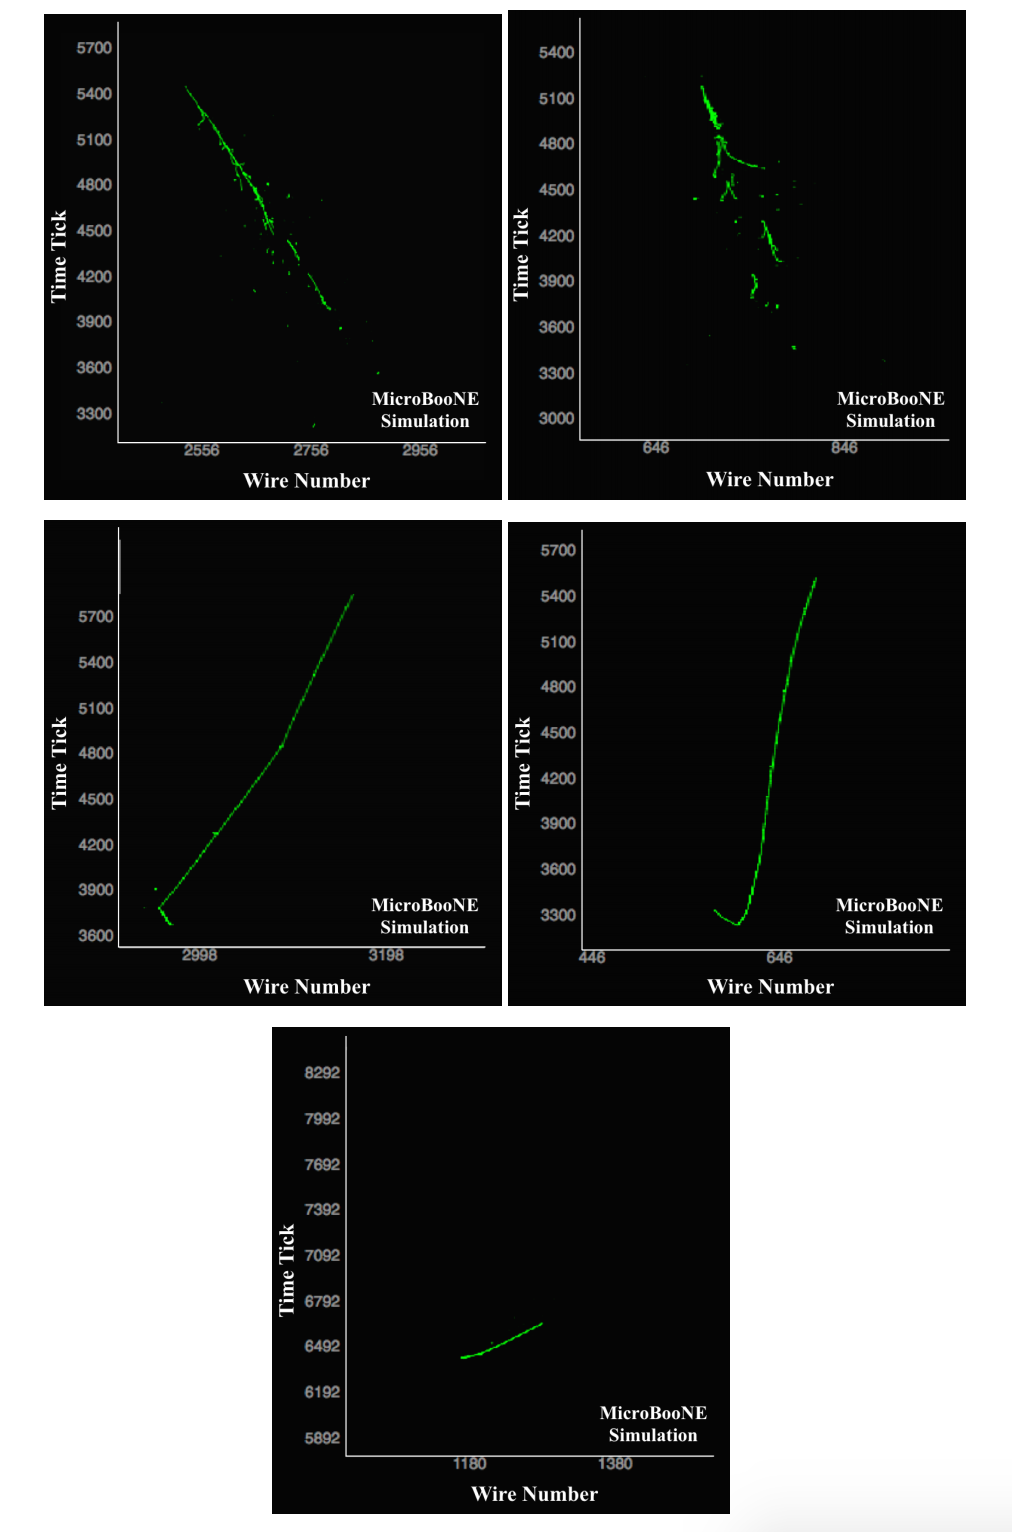
\includegraphics[width=0.8\textwidth]{Figures/five_part_types.png}

\caption{Example display for classification of each particle type in the collection plane.  From top left and moving clockwise: $e^-$, $\gamma$, $\mu^-$, proton, and $\pi^-$. (Should this cite previous paper again? Image?}
  \label{fig:fiveparts}
\end{figure}

%The tracks are mostly all contained in the fiducial volume.

\section{Image Preparation}

Throughout all studies in this work, we use one of the most popular open-source CNN software frameworks, {\sc{Caffe}}~\cite{caffe}, for CNN training and analysis. Input data is in a ROOT file format~\cite{ROOT} created by the {\sc{LArCV}} software framework~\cite{LArCV}, which we developed to act as the interface between {\sc{LArSoft}} and {\sc{Caffe}}. {\sc{LArCV}} is also an image data processing framework and is used to further process and analyze images as described in the following sections. One can find our custom version of {\sc{Caffe}} that utilizes the {\sc{LArCV}} framework in \cite{LArCV}.  
The computing hardware used in this study consists of multiple servers at various institutions. We have two dual-GPU 12 GByte memory, NVIDEA GPU servers of similar specifications at the Massachusetts Institute of Technology, Columbia University,  University of Michigan, Yale University. We also emply a DGX-1 10-GPU 18 GB/GPU server at Pacific Northwest National Laboratories.

... representative image picture here, as from the original CNN paper ... Figure \ref{fig:towerpower}

\begin{figure}[t]
  \centering  
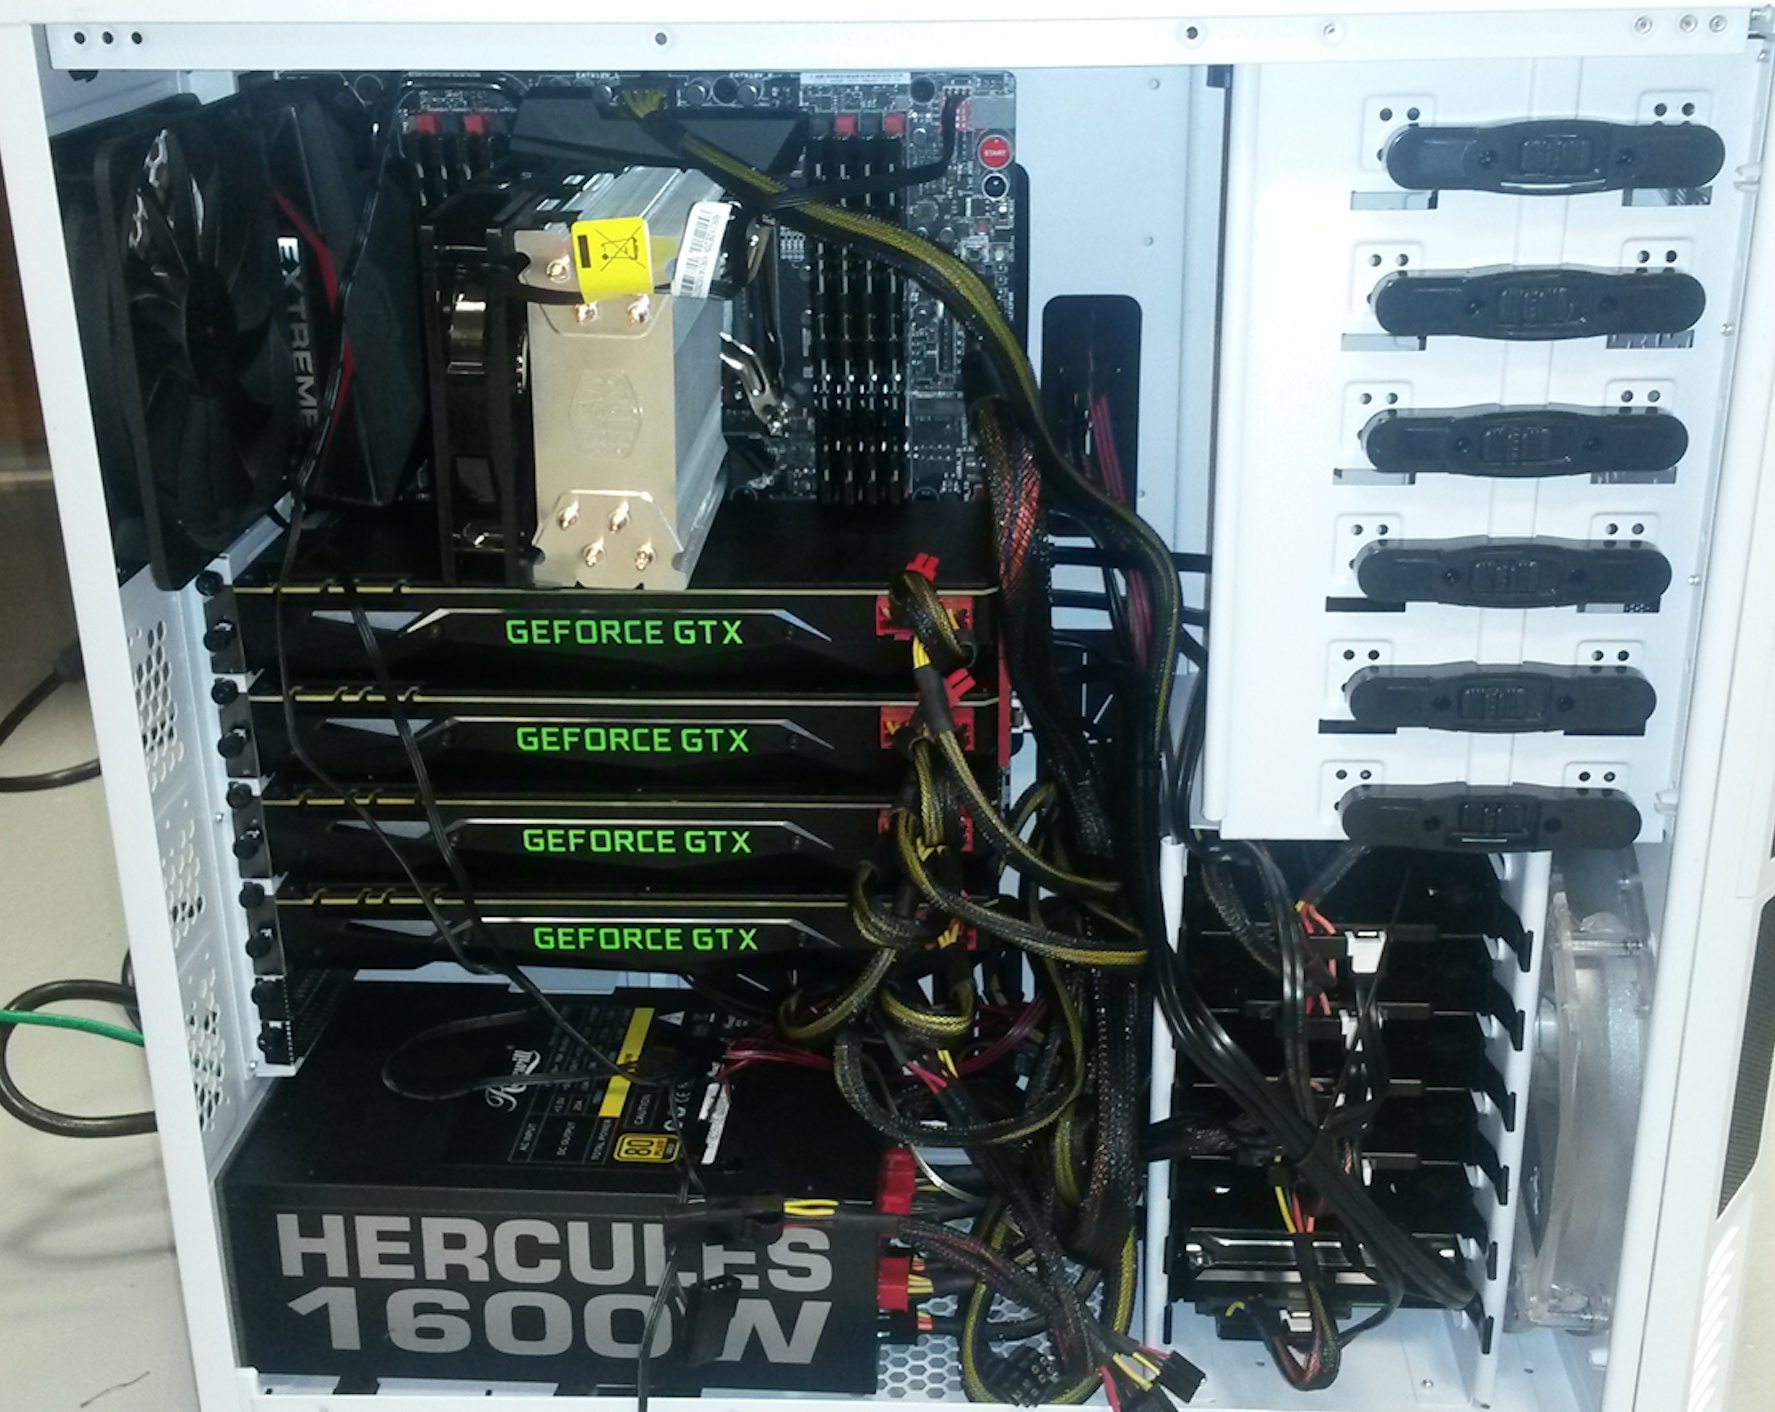
\includegraphics[width=0.495\textwidth]{Figures/tower_power.png}\\
\caption{One example of GPU tower employed in the training (is this the representative image referred to?)}
  \label{fig:towerpower}
\end{figure}


\section {Training and Inference}

A disciplined training and inference procedure is required in order to compare the performance of various networks. This procedure is as follows: First, we organize a training sample of 2000 events of each particle type. We additionally create 2 testing samples A and B: test A contain 10000 events and will be used to choose a weight file from the training, while test B contain 30000 and will be used for final performance reporting.  Our training uses a batch size of 20 images, and runs iteratively where the complete forward/backward pass through each batch marks an iteration. During this time, the testA set's loss curve is monitored. When the loss has achieved its global minimum and begins to rise again, such that this minimum is reached at 85\% or less of the total number of iterations, we stop training and note the iteration value. The goal is to ensure that learning has plateaued before we stop training. To ensure that the learning is stable at this observed minimum, we run the inference stage on the test A sample at the minimum iteration $\pm$ 5 epochs.  

The best inference run on a given epoch in test sample A is then identified as the weight file to be used in the final inference stage. This final inference in run on test sample B, and is used to extract final performance numbers.


\section {The Architectures}
%\subsection{Original CNN paper architectures}
Broad descriptions here of ResNet and Vgg16 and whatever else we have results for.  GoogleNet, AlexNet?
Why we want to stick with flavors of ResNet and Vgg here. Perhaps we don't want each flavor of ResNet and Vgg16 to be its own subsection.

\subsection{ResNet}
The first networks considered here are ResNet networks \cite{bib:resnet}. ResNets are made up primarily of residual convolutional modules, where each module represents a layer of the network. The general purpose of these modules is to preserve information learned in previous layers using an identity mapping, and to optimize from there. In other words, the modules refocus the network training from a function over feature space to to a residual of that function over feature space. Networks constructed from these modules have been shown to improve performance as network depth increases while also to decrease computational training time \cite{bib:resmodule}.  

\par ResNet is built on the idea that an increase in depth will lead to an increase in performance. For this reason, one of our primary goals here is to measure the computational costs of added depths to assess whether this depth is worth the extra resources it consumes. We additionally explore the width of the network and the addition of bottleneck feature (citation).  An example of inference results on the testA sample is shown in Figure \ref{fig:inferenceA}; the weight file used to calculate final performance on testB is extracted from this plot.  This weight file is then used to run inference on testB.  The results from this second inference run are shown in Table \ref{tab:classCompare}. Additional efficiency vs purity curves are shown in Figure \ref{fig:resneteffpur}.\\

\begin{figure}[t]
  \centering  
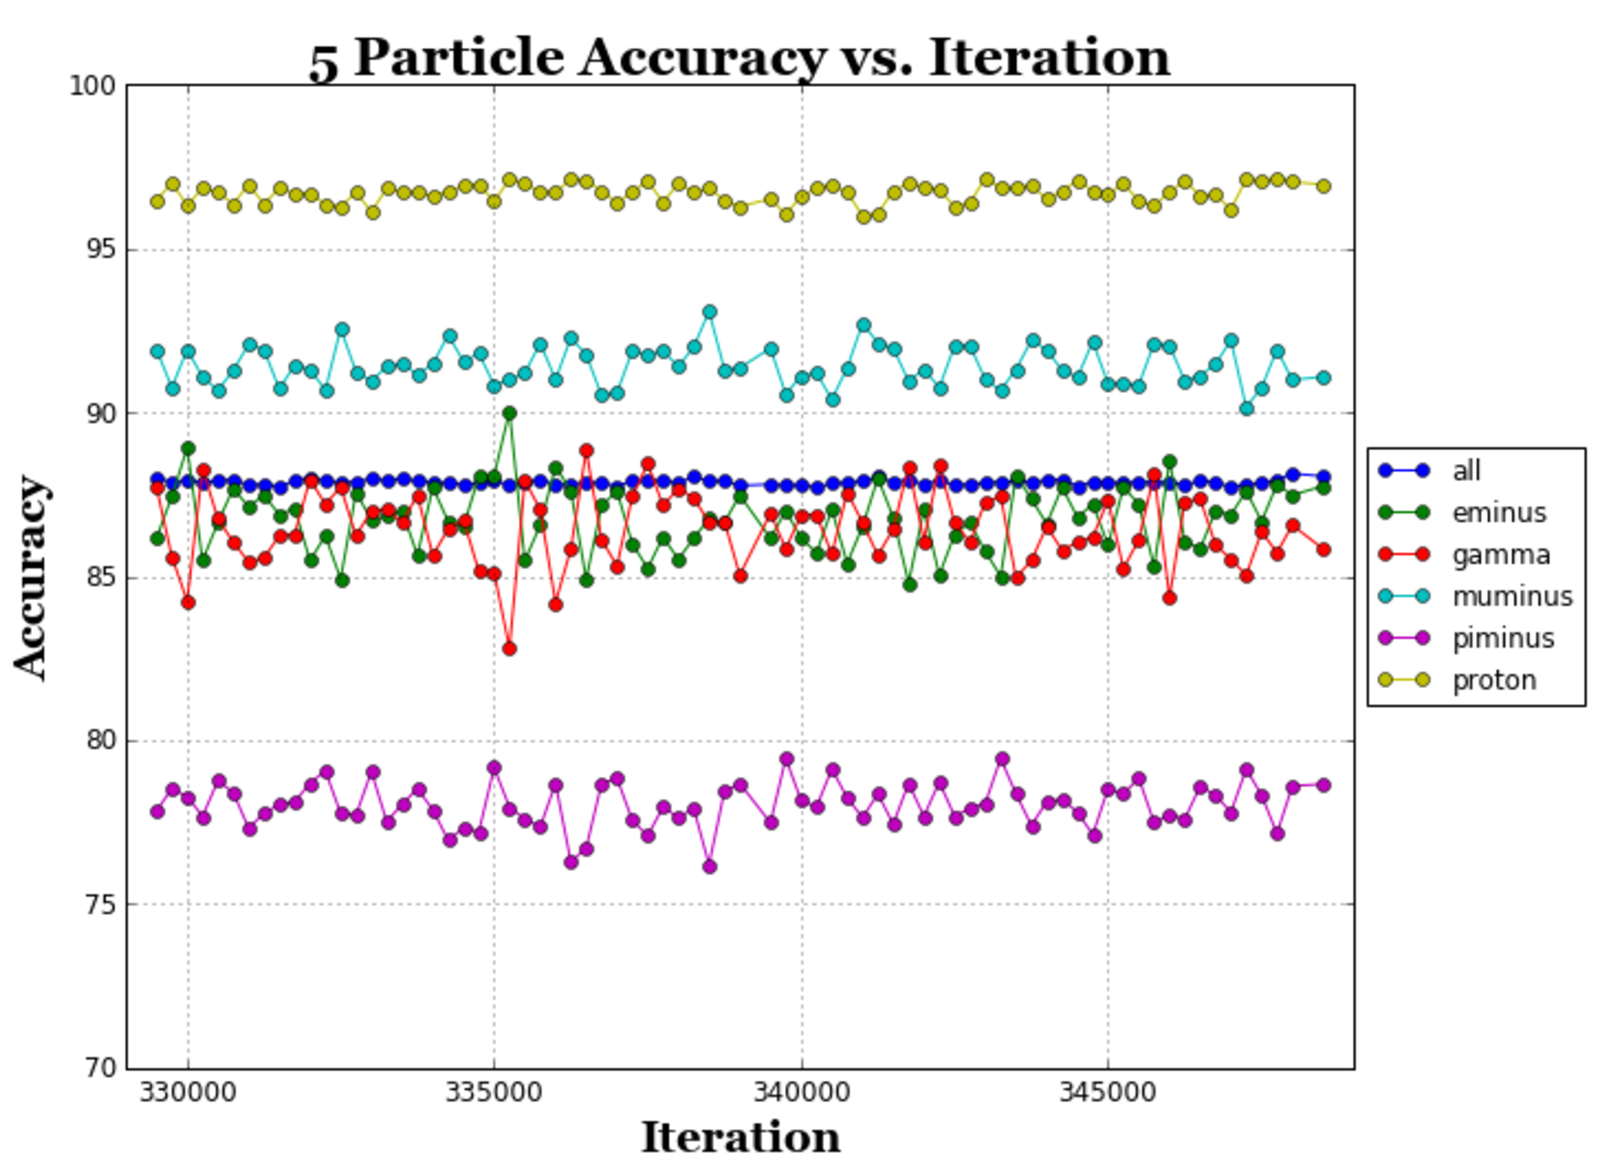
\includegraphics[width=0.6\textwidth]{Figures/testAinference.png}\\
\caption{Example of inference results on the testA sample for $\pm$ 5 epochs around global loss minimum. The weight file for final performance assessment on testB is chosen based on the point of overall maximum accuracy in this plot. }
  \label{fig:inferenceA}
\end{figure}

\par \noindent
\vspace{2 mm}
\begin{minipage}{\linewidth}
\centering
\captionof{table}{The right five columns denote the classification performance per particle type. Errors shown are statistical
and assume a binomial distribution. } \label{tab:classCompare} 
\begin{tabular}{clllll}
 & \multicolumn{5}{c}{Classified Particle Type} \\
\cline{2-6}
\vspace{-0.1in}\\
\vspace{0.05in}
Network & $e^-$ [\%] & $\gamma$ [\%] & $\mu^-$ [\%] & $\pi^-$ [\%] & proton [\%] \\
\hline 
\vspace{-0.1in}\\
\vspace{0.05in}
 VGG16a & 83.9 $\pm 0.2$ & 88.3 $\pm 0.2$  & 90.1 $\pm 0.2$ & 77.0 $\pm 0.2$ & 95.0 $\pm 0.1$ \\ 
 \vspace{0.05in}
 VGG16b & 83.8 $\pm 0.2$ & 90.0 $\pm 0.2$  & 92.0 $\pm 0.2$ & 79.0 $\pm 0.2$ & 96.2 $\pm 0.1$ \\ 
 \vspace{0.05in}
 VGG16c & 85.9 $\pm 0.2$ & 87.8 $\pm 0.2$  & 89.9 $\pm 0.2$ & 81.0 $\pm 0.2$ & 95.1 $\pm 0.1$ \\ 
 \vspace{0.05in}
 ResNet14b & 84.8 $\pm 0.2$ & 85.0 $\pm 0.2$  & 90.5 $\pm 0.2$ & 76.0 $\pm 0.2$ & 94.0 $\pm 0.1$ \\ 
 \vspace{0.05in}
 ResNet29b & 87.2 $\pm 0.2$ & 86.7 $\pm 0.2$  & 90.7 $\pm 0.2$ & 78.8 $\pm 0.2$ & 96.8 $\pm 0.1$ \\ 
 \vspace{0.05in}
 ResNet29b\_w4 & 87.9 $\pm 0.2 $ & 86.0 $\pm 0.2$  & 90.6 $\pm 0.2$ & 78.9 $\pm 0.2$ & 96.2 $\pm 0.1$ \\ 
 \vspace{0.05in}
 ResNet50b & 87.7 $\pm 0.2$ & 85.9 $\pm 0.2$  & 93.1 $\pm 0.1$ & 78.5 $\pm 0.2$ & 96.2 $\pm 0.1$ \\ 

 \vspace{0.05in}

 PlainResNet10b & 84.7 $\pm 0.2$ & 84.5 $\pm 0.2$  & 91.0 $\pm 0.1$ & 75.8 $\pm 0.2$ & 96.1 $\pm 0.1$ \\ 
 \vspace{0.05in}
 PlainResNet10b\_w4 & 85.6 $\pm 0.2$ & 85.6 $\pm 0.2$  & 91.5 $\pm 0.2$ & 78.3 $\pm 0.2$ & 96.3 $\pm 0.1$ \\ 
 \vspace{0.05in}
 PlainResNet12b & 84.5 $\pm 0.2$ & 85.1 $\pm 0.2$  & 92.6 $\pm 0.2$ & 74.4 $\pm 0.3$ & 95.4 $\pm 0.1$ \\ 
 \vspace{0.05in}
 PlainResNet18b & 85.5 $\pm 0.2$ & 85.9 $\pm 0.2$  & 93.1 $\pm 0.1$ & 78.5 $\pm 0.2$ & 96.2 $\pm 0.1$ \\ 
 \vspace{0.05in}
 PlainResNet18b\_w4 & 82.3 $\pm 0.2$ & 81.4 $\pm 0.2$  & 85.9 $\pm 0.2$ & 73.4 $\pm 0.3$ & 91.6 $\pm 0.2$ \\ 
 \vspace{0.05in}
 PlainResNet20b & 90.4 $\pm 0.2$ & 81.2 $\pm 0.2$  & 88.0 $\pm 0.2$ & 77.1 $\pm 0.2$ & 95.6 $\pm 0.1$ \\ 
 \vspace{0.05in}
 PlainResNet20b\_w4 & 72.2 $\pm 0.3$ & 74.9 $\pm 0.3$  & 72.1 $\pm 0.3$ & 73.2 $\pm 0.3$ & 80.0 $\pm 0.2$ \\ 
 \vspace{0.05in}
 \vspace{0.05in}
    \end{tabular}
\end{minipage}

\par \noindent
\vspace{2 mm}
\begin{minipage}{\linewidth}
\centering
\captionof{table}{Computational performance for various ResNet architectures} \label{tab:resnetComput} 
\begin{tabular}{cllllll}
 & \multicolumn{5}{c}{THESE NUMBERS CURRENTLY WRONG} \\
\cline{2-6}
\vspace{-0.1in}\\
\vspace{0.05in}
Network & Mem (MB) & Wall Time (s) & IO Wait Time (s) & IO Thread Time (s) & IO Thread Copy Time & Caffe Copy Time(s) [\%] \\
\hline 
\vspace{-0.1in}\\
\vspace{0.05in}
 ResNet14b & 84.8 $\pm 0.2$ & 85.0 $\pm 0.2$  & 90.5 $\pm 0.2$ & 76.0 $\pm 0.2$ & 94.0 $\pm 0.1$ & 0. \\ 
 \vspace{0.05in}
 ResNet29b & 87.2 $\pm 0.2$ & 86.7 $\pm 0.2$  & 90.7 $\pm 0.2$ & 78.8 $\pm 0.2$ & 96.8 $\pm 0.1$ & 0 \\ 
 \vspace{0.05in}
 ResNet29b\_w4 & 87.9 $\pm 0.2 $ & 86.0 $\pm 0.2$  & 90.6 $\pm 0.2$ & 78.9 $\pm 0.2$ & 96.2 $\pm 0.1$ & 0 \\ 
 \vspace{0.05in}
 ResNet50b & 87.7 $\pm 0.2$ & 85.9 $\pm 0.2$  & 93.1 $\pm 0.1$ & 78.5 $\pm 0.2$ & 96.2 $\pm 0.1$ & 0\\ 
 \vspace{0.05in}
    \end{tabular}
\end{minipage}

\begin{figure}[t]
  \centering  
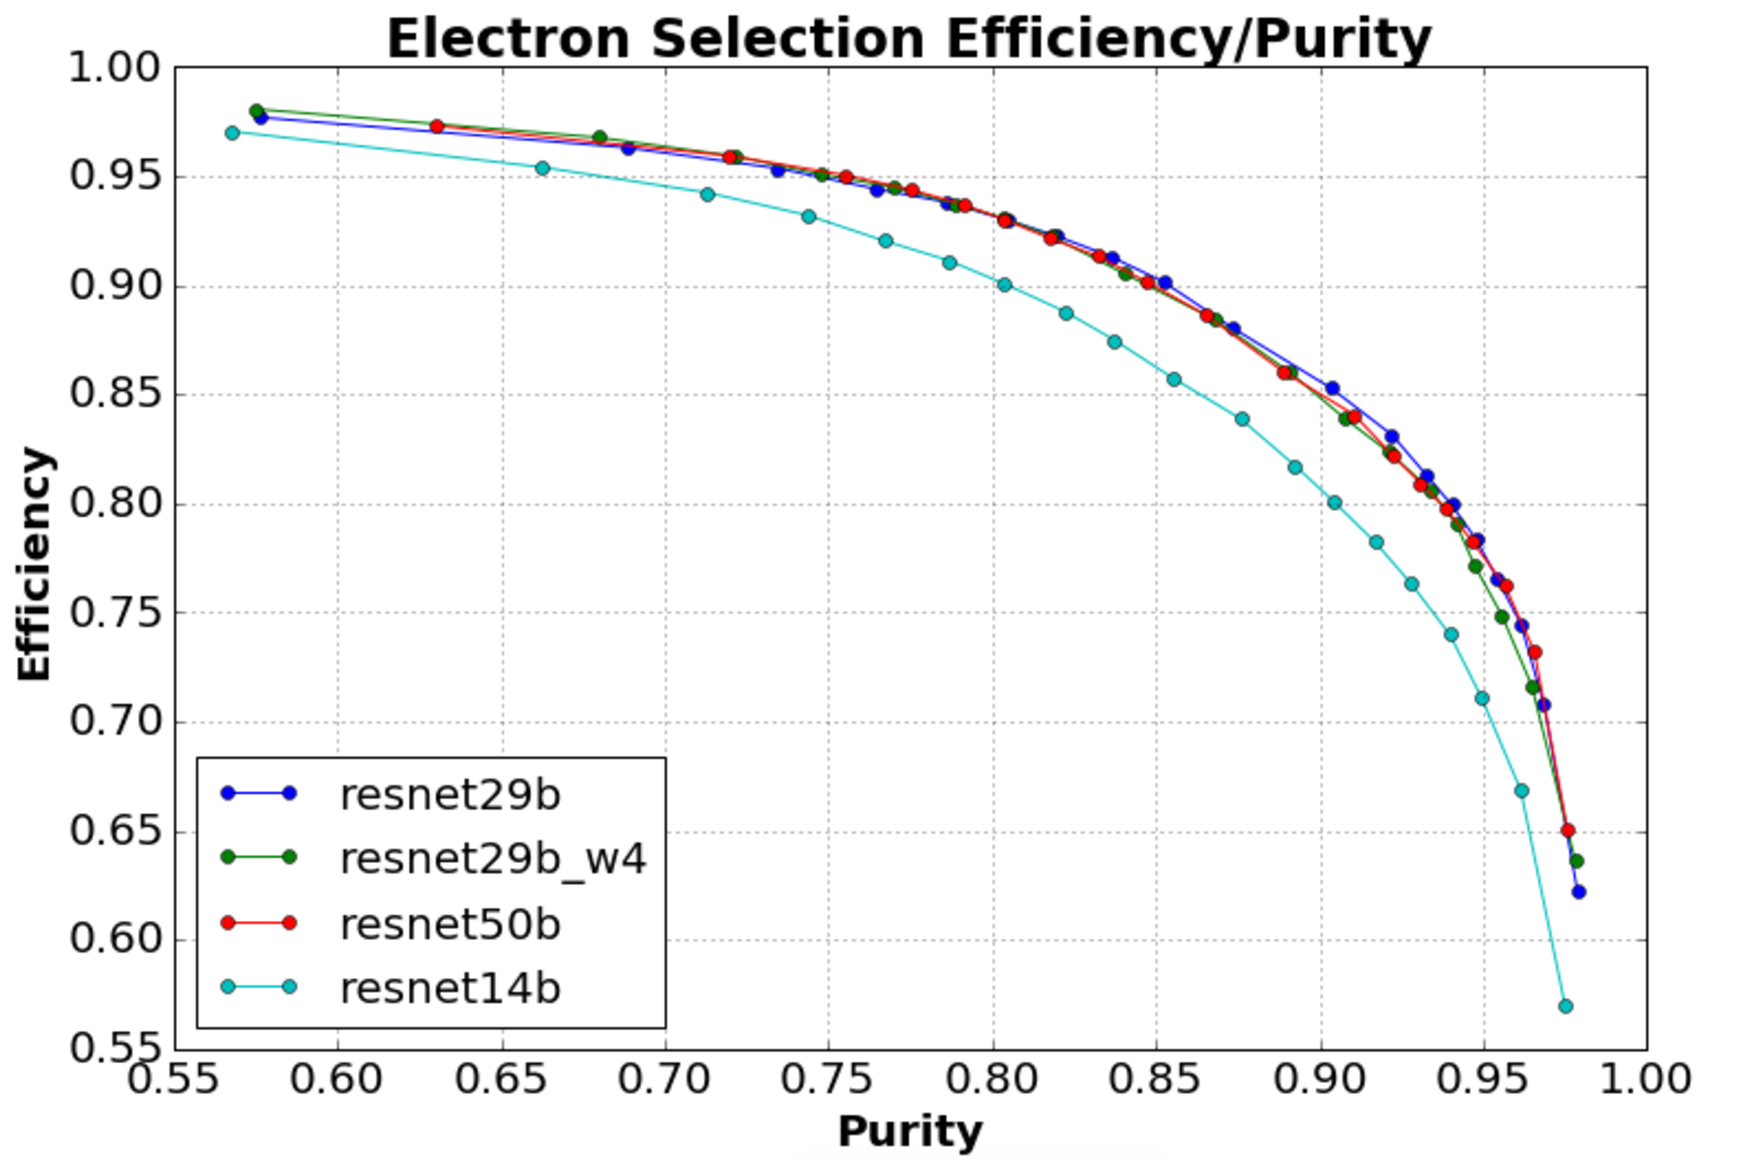
\includegraphics[width=0.45\textwidth]{Figures/resnet_effpur.png}
\hspace{2 mm}
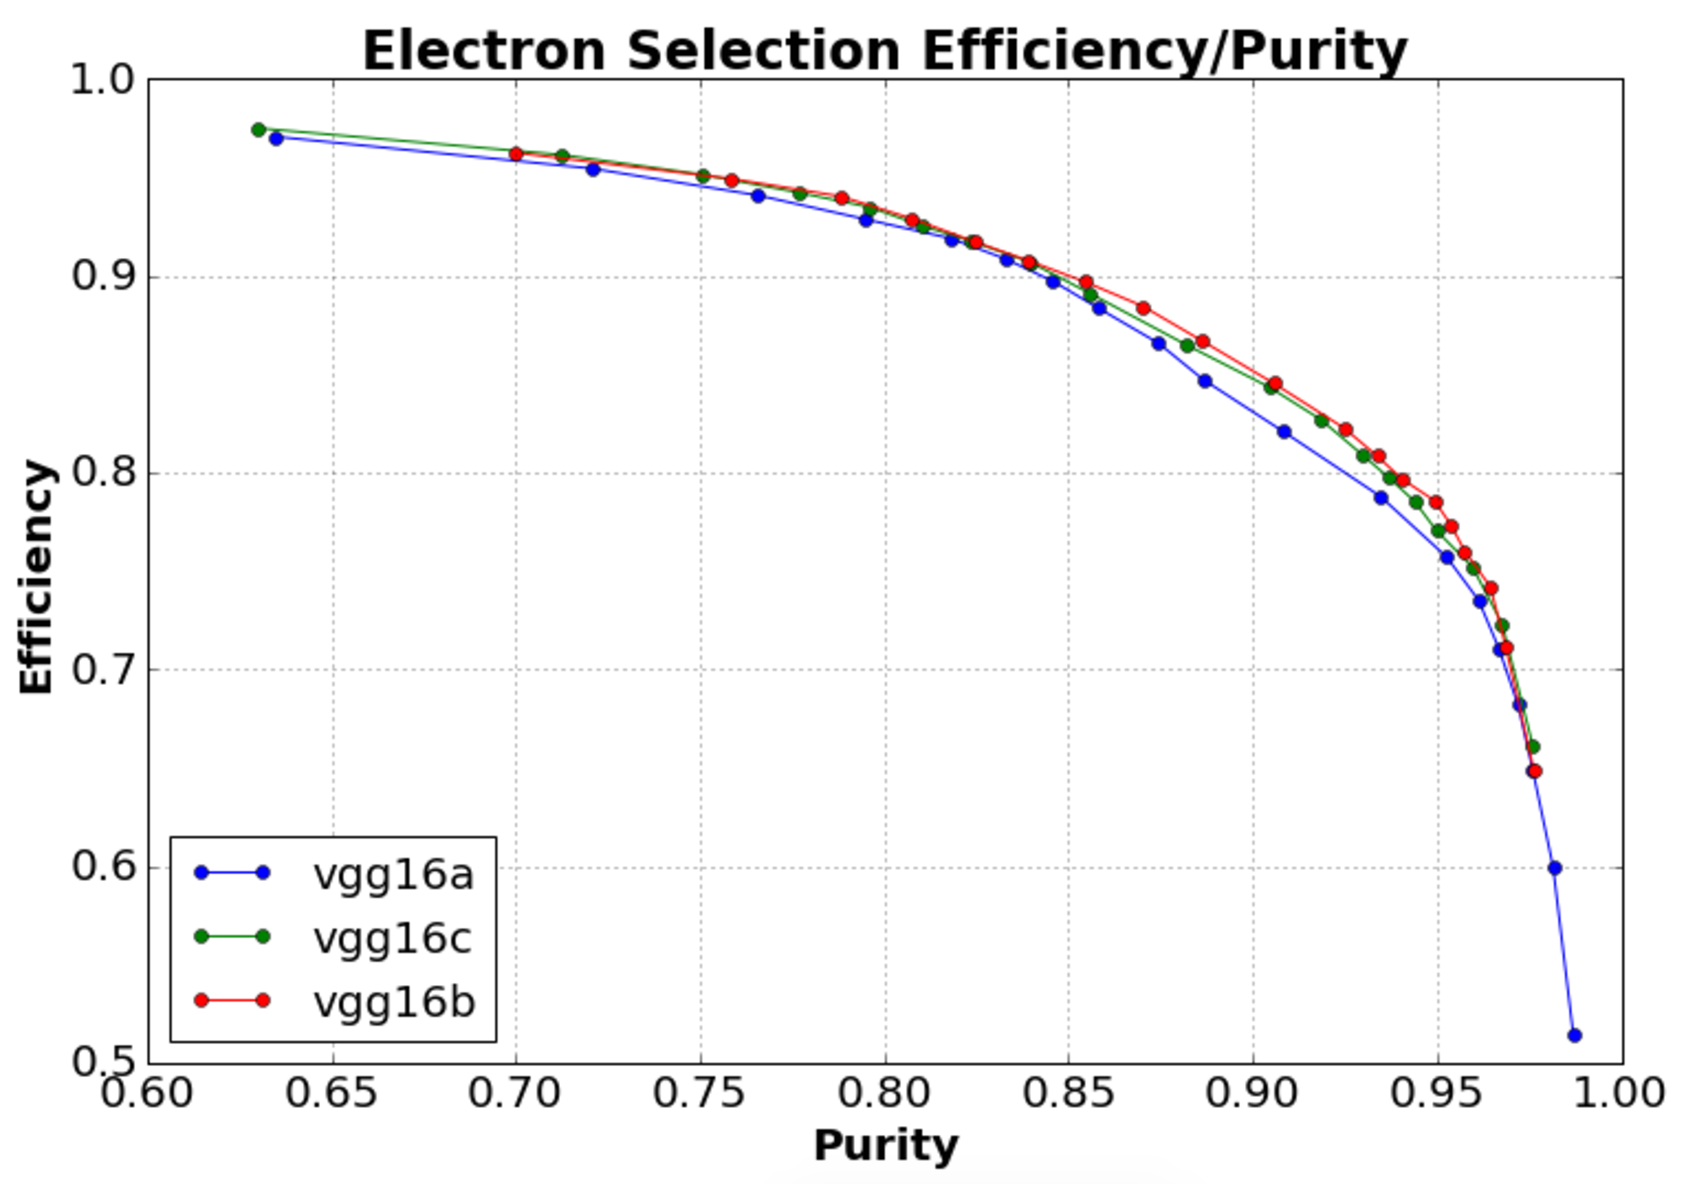
\includegraphics[width=0.45\textwidth]{Figures/vgg_effpur.png}\\
\caption{a) Efficiency vs purity curves for all resnet networks.  As expected, ResNet14b is on the lower end, while the others are fairly comparable (left). b) Efficiency vs purity for all VGG nets (right). }
  \label{fig:resneteffpur}
\end{figure}

\begin{figure}[t]
  \centering  
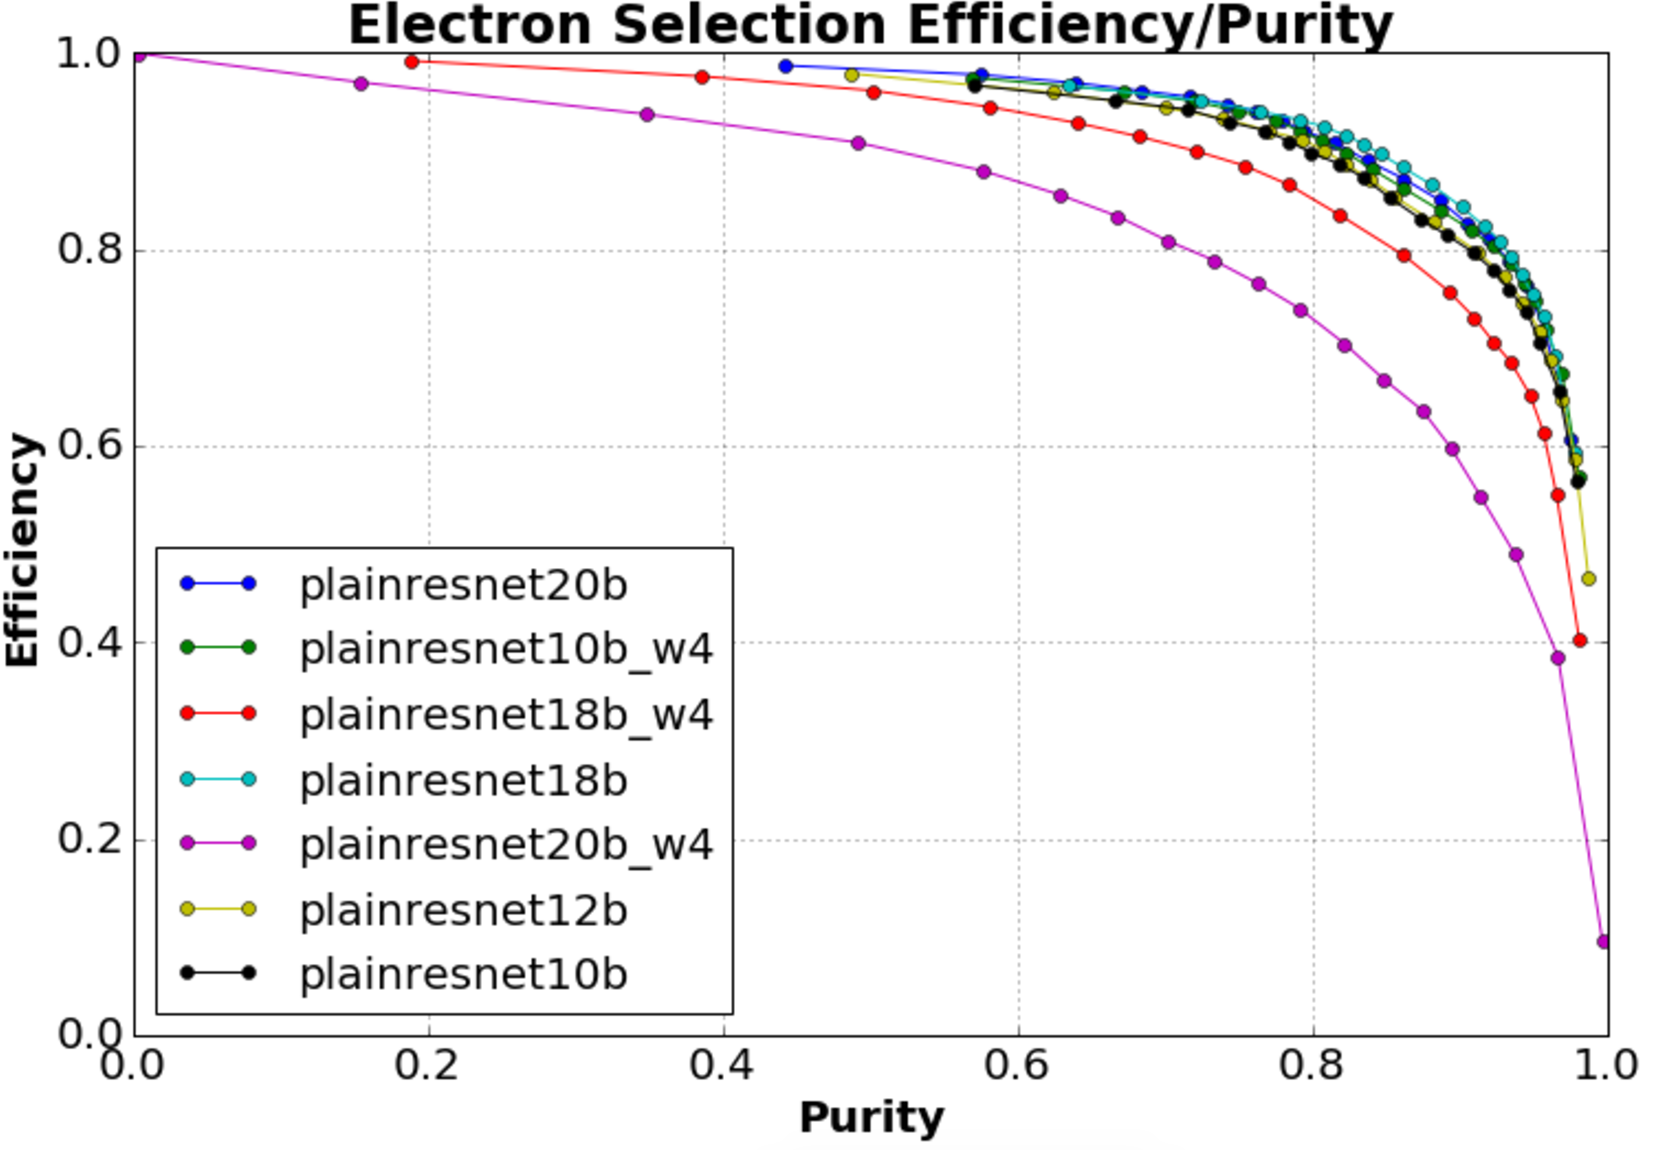
\includegraphics[width=0.45\textwidth]{Figures/plainresnet_effpur.png}
\hspace{2 mm}
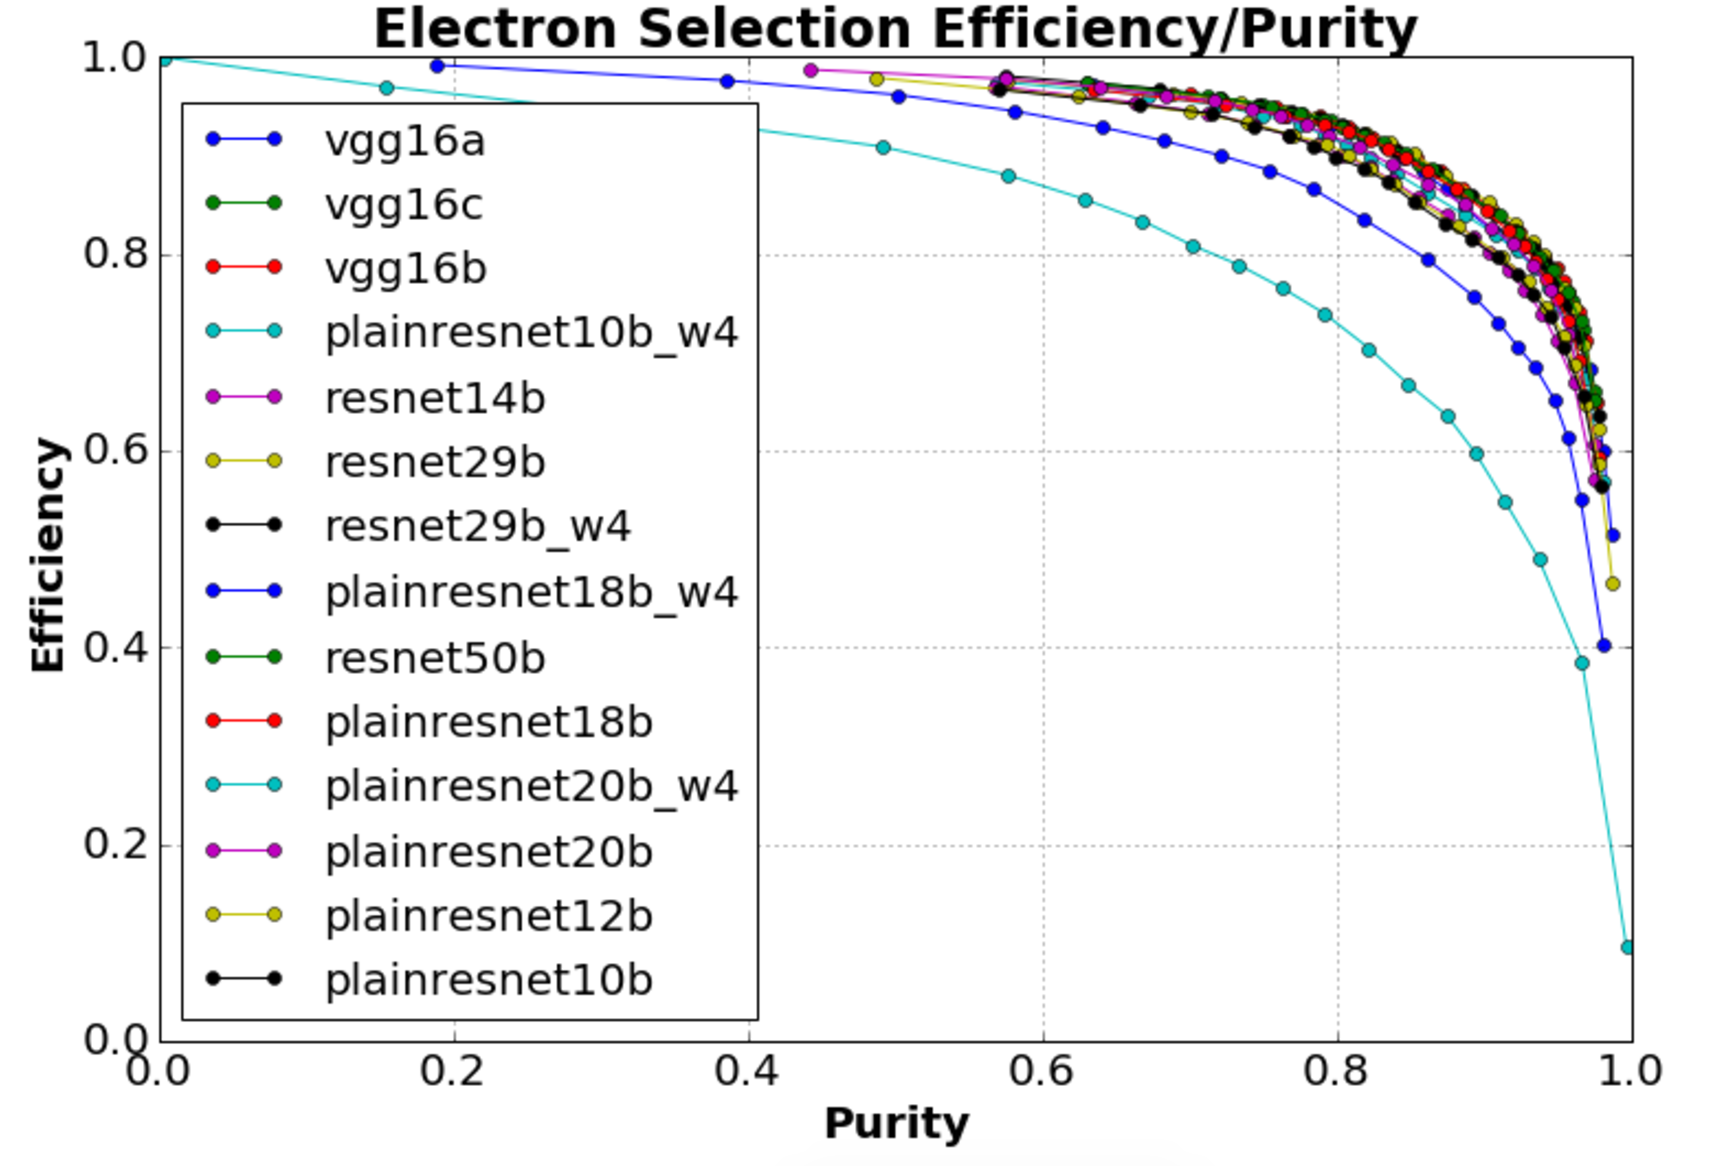
\includegraphics[width=0.45\textwidth]{Figures/all_effpur.png}\\
\caption{a) Efficiency vs purity curves for all plainresnet networks (left). b) Efficiency vs purity for all nets (right). }
  \label{fig:plainresneteffpur}
\end{figure}

%\begin{figure}[t]
%  \centering  
%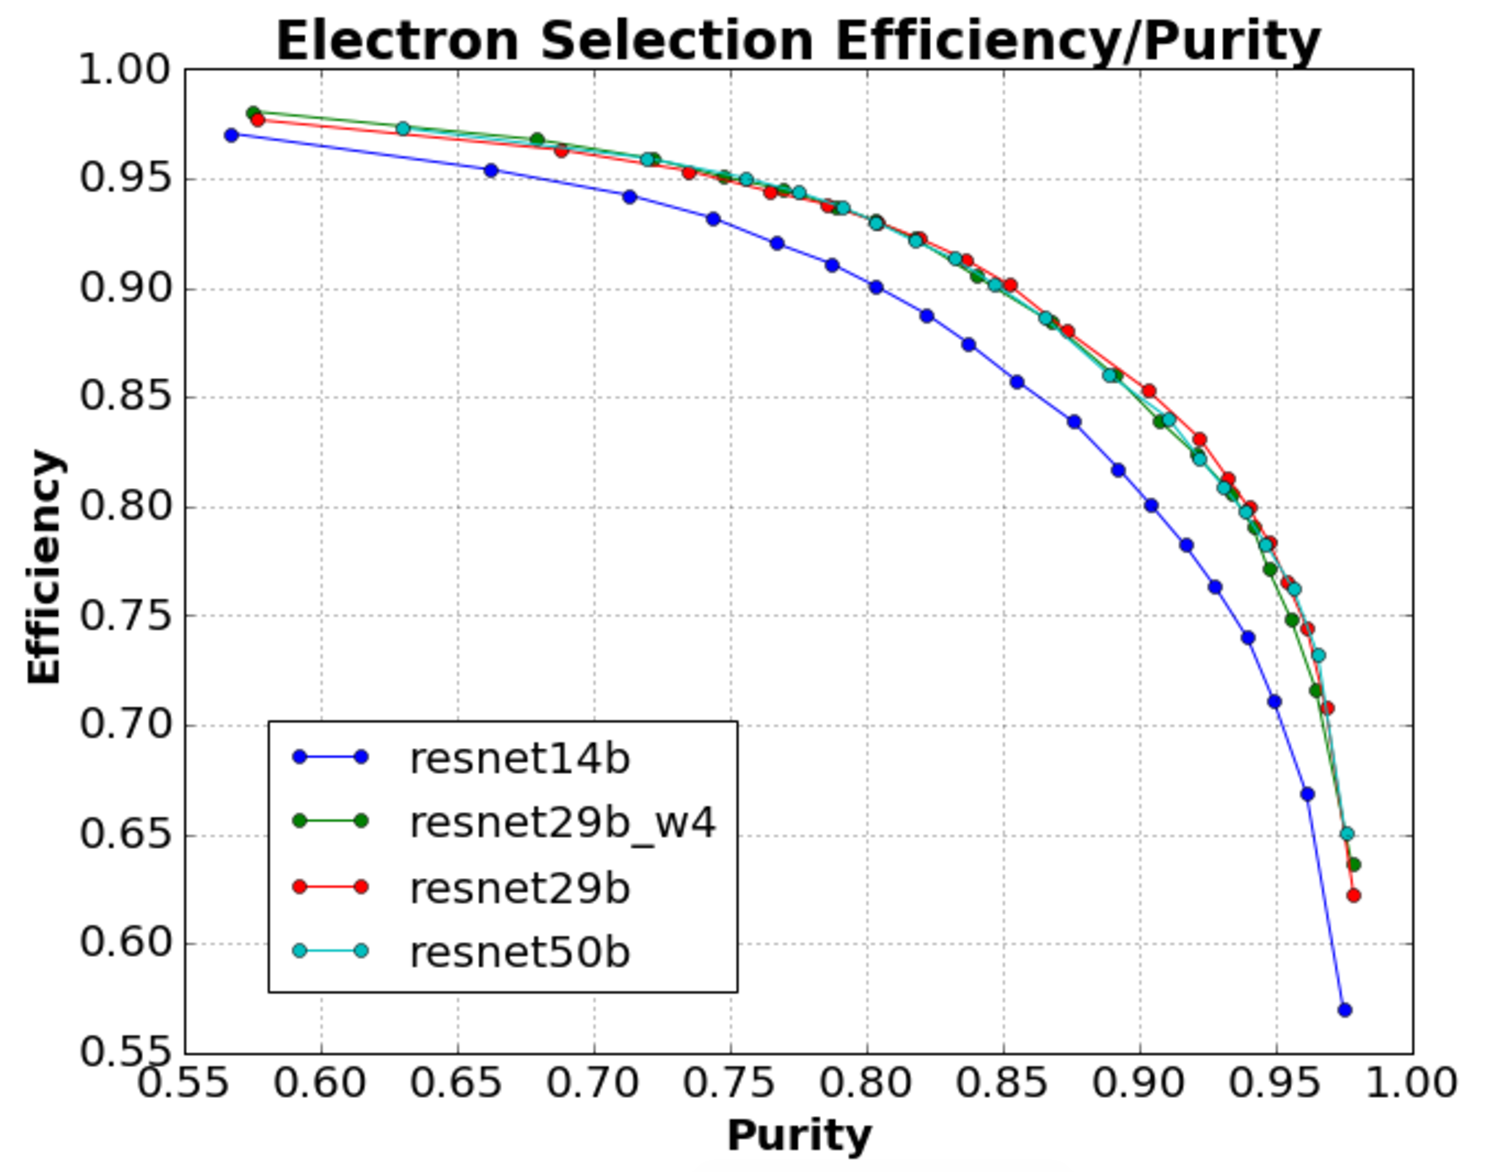
\includegraphics[width=0.6\textwidth]{Figures/resneteffpur.png}\\
%\caption{Efficiency vs purity curves for all resnet networks.  As expected, ResNet14b is on the lower end, while the others are fairly comparable. }
%  \label{fig:resneteffpur}
%\end{figure}



\par From Table \ref{tab:classCompare} and Table \ref{tab:resnetComput} we can conclude several things.  First, we see that in general, performance increases as depth increase.  (We seee from Kevin's slides that resources usage also increases with depth). From the Resnet29b\_w4 results we see that increasing the width of the Resnet results in minimal performance increase at the high cost of computational resources.  We also see that the bottleneck architecture increases performance minimally at the expense of resources (from Kevin's slides).  We conclude here that resnet29 is the best choice of the ResNet in terms of computational and overall performance.  

\subsection{VGG}


{\color{red} Not to be included, but for convenience, all results are\/should-be referenced at 
\begin{verbatim}https://docs.google.com/presentation/d/1Rvo2Yt9KqRQk2eDyO1WeA5GwaWamLvZR2CR3txfYbBE/edit#slide=id.g1ec338afdf_0_11. We probably don't want to exhaustively provide all plots for all networks ...
\end{verbatim}
}

%\subsection{ResNet14b}
%\subsection{ResNet14b\_w2}
%\subsection{vgg16a}
%\subsection{vgg16b}

\begin{figure}[t]
  \centering  
\begin{subfigure}[t]{0.45\textwidth}
\centering
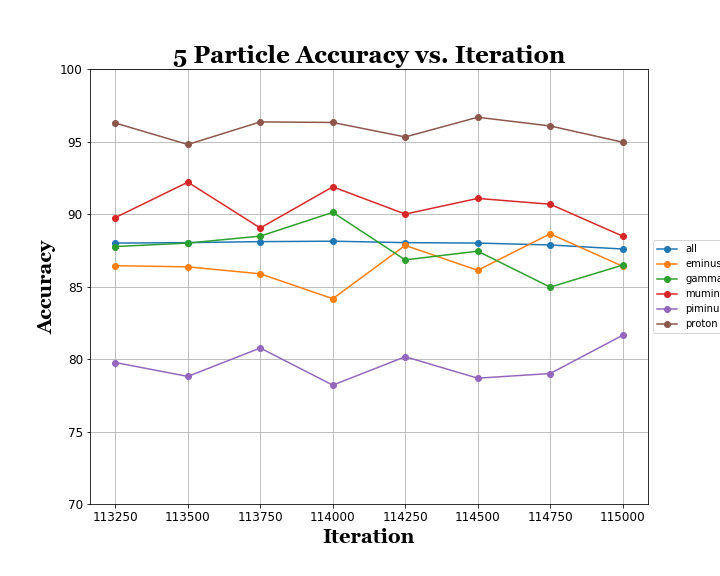
\includegraphics[width=\textwidth]{../vgg16b/part5_vggb.png}
\label{a}
\caption{The Accuracy for 5 species classification}
\end{subfigure}%
\hfill
\begin{subfigure}[t]{0.45\textwidth}
\centering
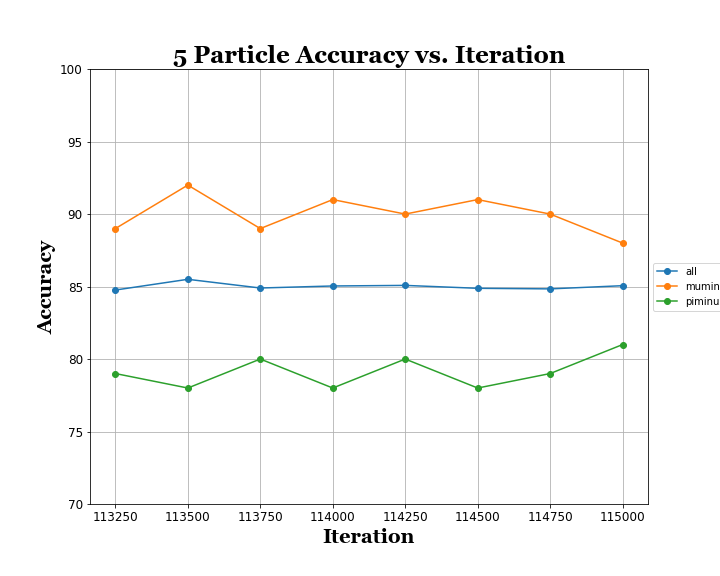
\includegraphics[width=\textwidth]{../vgg16b/part_mu-pi_vggb.png}
\label{b}
\caption{$\mu/\pi$ classification.}
\end{subfigure}%

\bigskip

\begin{subfigure}[t]{0.45\textwidth}
\centering
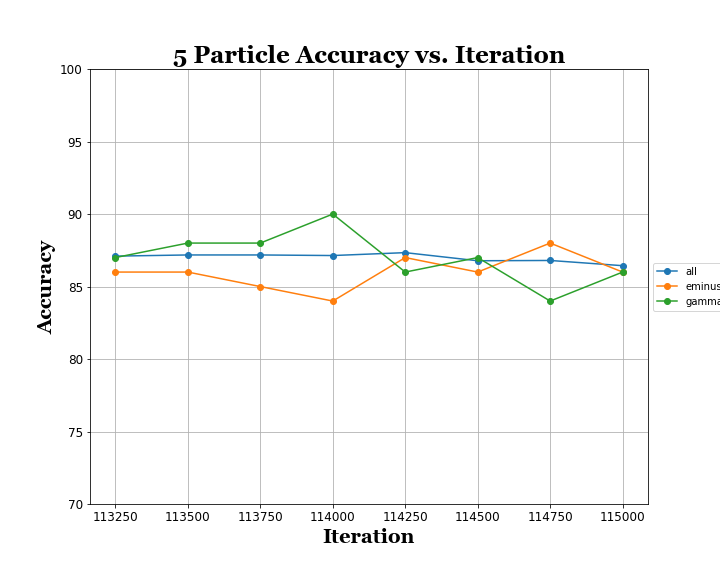
\includegraphics[width=\textwidth]{../vgg16b/part_e-gamma_vggb.png}
\label{c}
\caption{$e/\gamma$ classification}
\end{subfigure}%
\hfill
\begin{subfigure}[t]{0.45\textwidth}
\centering
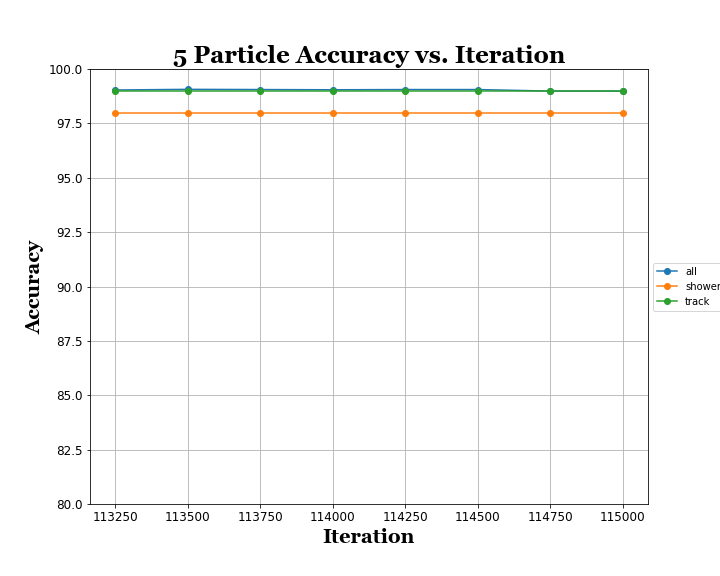
\includegraphics[width=\textwidth]{../vgg16b/part_show-trk_vggb.png}
\label{d}
\caption{$e/\gamma$ versus $\mu,\pi,p$ classification}
\end{subfigure}%
\caption{This is the (a) five particle classification, and (b) $\mu^-/\pi^-$, (c) $e/\gamma$, and (d) shower/track separations for the vgg16b network.}
\label{fig:vgg16b}
\end{figure}
%\subsection{vgg16c}


\section {Conclusions}

We have surveyed a variety of CNNs for the sake of classifying five charged particles as they appear in LArTPCs. Some interesting conclusions are that while Ref.~\cite{uB-JINST} achieved formidable performance, a few other networks do as well or better, and it is seen now that RestNetXYZ and VGG16XYZ are better choices.

We plan to start with these networks for future physics-identification tasks in MicroBooNE; we believe similar guidance for general TPCs applies there, as well. We advocate, per this study, that the full and infinite (hyper) parameter space for CNNs need not be explored in those future analyses in favor of the identified best-performing networks here.

%\appendix

%% Appendix 3: Bibliography %%
\newpage
%\section{Bibliography and References Cited}
%\bibliographystyle{JHEP}%{unsrt}
%\bibliography{arch}
\begin{thebibliography}{9}

\bibitem{AlexNet}
  Alex Krizhevsky {\it et al. },
  ``Imagenet Classification with Deep Convolutional Neural Networks,''
  \emph{NIPS} \textbf{25}, pages 1106–1114, 2012.

%MicroBooNE CNN JINST article \cite{ubooneCNN}
\bibitem{uB-JINST}
R. Acciarri {\it et. al.} [MicroBooNE collaboration],
"Convolutional Neural Networks Applied to Neutrino Events in a Liquid Argon Time Projection Chamber,"
\emph{1611.05531"} [phsics.ins-det].

\bibitem{SBN}
R. Acciarri {\it et al.} [SBN Collaboration],
``A Proposal for a Three Detector Short-Baseline Neutrino Oscillation Program in the Fermilab Booster Neutrino Beam,''
\emph{arXiv:1503.01520} [physics.ins-det].

\bibitem{DUNE}
R.~Acciarri {\it et al.} [DUNE Collaboration],
  ``Long-Baseline Neutrino Facility (LBNF) and Deep Underground Neutrino Experiment (DUNE) : Volume 1: The LBNF and DUNE Projects,''
  \emph{arXiv:1601.05471} [physics.ins-det].

\bibitem{dayabay}
E. Racah {\it et al.} ``Revealing Fundamental Physics from the Daya Bay Neutrino Experiment using Deep Neural Networks,'' \emph{arXiv:1601.07621}.

\bibitem{nova}
A. Aurisano {\it et al.}, ``A Convolutional Neural Network Neutrino Event Classifier,'' 2016 \emph{JINST} 11 P09001.

\bibitem{NEXT}
J.~Renner {\it et al.} [NEXT Collaboration],
``Background rejection in NEXT using deep neural networks,''
\emph{arxiv:1609.06202}.

\bibitem{larsoft050800}
LArSoft release {\it redmine} \textbf{05.08.00} \protect\url{https://cdcvs.fnal.gov/redmine/projects/larsoft/wiki/ReleaseNotes050800}.

\bibitem{uboonecode050800}
uboonecode release {\it redmine} \textbf{05.08.00} \protect\url{https://cdcvs.fnal.gov/redmine/projects/uboonecode/wiki/ReleaseNotes050800}.

\bibitem{LArCV}
 Genty, Terao and Wongjirad, LArCV: LArTPC Image Processing/Analysis Framework for Deep Learning \protect\url{https://www.github.com/LArbys/LArCV} %\protect\url{http://microboone-docdb.fnal.gov:8080/cgi-bin/ShowDocument?docid=5847}
 
\bibitem{caffe}
 Y. Jia {\it et al.}, ``Caffe: Convolutional Architecture for Fast Feature Embedding,'' {\emph arXiv:1408.5093}, 2014.
 
\bibitem{GoogLeNet}
Christian Szegedy {\it et al.}, ``Going Deeper with Convolutions,''
  \emph{arXiv:1409.4842}, 2014.

\bibitem{fasterrcnn}
Ren, Shaoqing and He, Kaiming and Girshick, Ross and Sun, Jian,
``Faster R-CNN: Towards Real-Time Object Detection with Region Proposal Networks,''
\emph{NIPS} \textbf{28} pages 91-99, 2015.

\bibitem{Inceptionv4}
Szegedy {\it et al.}, ``Inception-v4, Inception-ResNet and the Impact of Residual Connections on Learning,'' \emph{arXiv:1602.07261}.

\bibitem{ResNet}
  Kaiming He {\it et al.}, ``Deep Residual Learning for Image Recognition,'' \emph{arXiv:1512.03385}.

\bibitem{ROOT}
Rene Brun and Fons Rademakers,
``ROOT -- An object oriented data analysis framework,''
{\it NIM} {\bf A389} 81-86, 2015.

\bibitem{titanx}
NVIDIA GeForce Titan X GPU Card Specification, \protect\url{http://www.geforce.com/hardware/desktop-gpus/geforce-gtx-titan-x/specifications}

\bibitem{geant4}
S. Agostinelli {\it et al.}, ``GEANT4: A Simulation toolkit,''
{\it NIM} {\bf A506} 250-303, 2003.

\bibitem{ubnoisefiltering}
MicroBooNE Collaboration, ``TPC Noise Filtering,'' MicroBooNE Public Note 1016-PUB.
\protect\url{http://www-microboone.fnal.gov/publications/publicnotes/index.html}

\bibitem{ubsignalprocessing}
MicroBooNE Collaboration. ``TPC Signal Processing,'' MicroBooNE Public Note 1017-PUB.
\protect\url{http://www-microboone.fnal.gov/publications/publicnotes/index.html}

\bibitem{backprop}
Montavon {\it et al.}, ``Neural Networks: Tricks of the Trade,'' Springer 2012.

\bibitem{BNB}
A. A. Aguilar-Arevalo {\it et al.}, ``The Neutrino Flux Prediction at MiniBooNE,'' \emph{PRD} \textbf{78}, 072002, 2009

\bibitem{genie}
C. Andreopoulos {\it et al.}, ``The GENIE Neutrino Monte Carlo Generator,''
{it NIM} {\bf A614} 87-104, 2010.
  
\bibitem{BatchNorm}
  Ioffe {\it et al.}, ``Batch Normalization: Accelerating Deep Network Training by Reducing Internal Covariate Shift,'' Proc. of the 32nd Intl. Conf. on Machine Learning 37, 2015.

\bibitem{dropout}
  Srivastava  {\it et al.}, ``Dropout: A Simple Way to Prevent Neural Networks from Overfitting,'' Journal of Machine Learning Research 15 1929-1958, 2014.

\bibitem{alphago}
D. Silver {\it et al.}, ``Mastering the game of Go with deep neural networks and tree search,'' Nature 529, 484–489, 2016.

\bibitem{rmsprop}
Tieleman, Tijmen and Hinton, Geoffrey. ``Lecture 6.5-rmsprop: Divide the gradient by a running
average of its recent magnitude,'' COURSERA: Neural Networks for Machine Learning, 4, 2012.

\bibitem{ccnote}
  MicroBooNE Collaboration, ``Selection and kinematic properties of $\nu_\mu$ charged-current inclusive events in 5e19 POT of MicroBooNE data,''
  \protect\url{http://www-microboone.fnal.gov/publications/publicnotes/MICROBOONE-NOTE-1010-PUB.pdf}

\bibitem{stabilitytraining}
  Zheng {\it et al.}, ``Improving the Robustness of Deep Neural Networks via Stability Training,'' \emph{arXiv:1604.04326}.

\bibitem{bib:resmodule}
Szegedy {\it et al.}, ``Inception-v4, Inception-ResNet and the Impact of Residual Connections on Learning,'' \emph{arXiv:1602.07261}.

\bibitem{bib:resnet}
Kaiming He {\it et al.}, ``Deep Residual Learning for Image Recognition,'' \emph{arXiv:1512.03385}.

\end{thebibliography}
\end{document}
